\chapter{The Menthal Backend (Speed) Architecture}
\label{chap:menthal_backend_architecture}

TODO: introduction

\section{Requirements analysis [SP]}
To determine the Menthal functional and non-functional requirements, first of all we need to formulate its use cases.
Figure~\ref{fig:menthal_use_case_diagram} represents the Use case diagram of Menthal project.
The system consists of two main parts, the client and the server.
This already gives a separation among its users.
On the one side, a user interact with a client application.
Menthal tracks the user behavior and provides a feedback, that is based on the gathered data analysis.
On the other side, system administrators and scientists interact with a server part.
Scientists carry on researches, analysing the obtained information.
A system administrator maintains the system, controls event processing and performes new analysis required by scientists.

\begin{figure}[h]
  \centering
  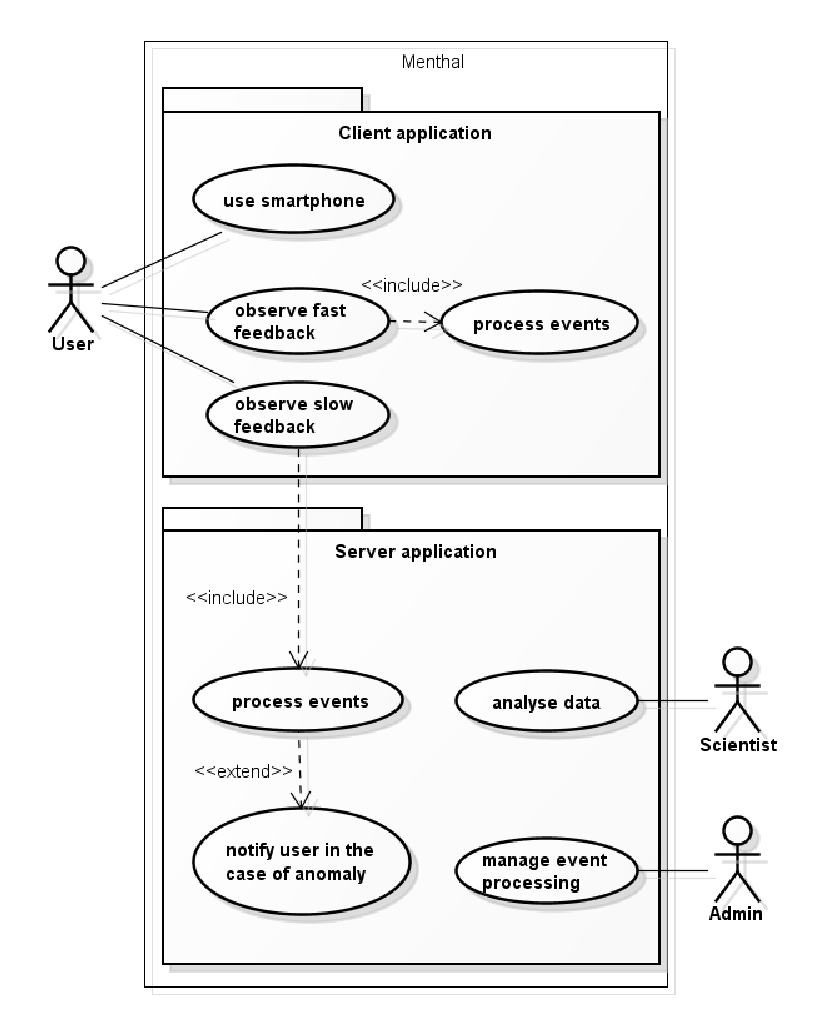
\includegraphics [width=0.9\textwidth]{images/menthal_use_case_diagram}
  \caption{Menthal Use case diagram}
  \label{fig:menthal_use_case_diagram}
\end{figure}


\subsection{Functional requirements}
% to analyze speed layer architecture
The scope of our work is a part of Lambda Architecture named a Speed Layer.
% it consists o three components
% three parts for: receivivg data, ..
It requires to implement three main parts: data receiving part, real-time data processing and the store of the results of computations.
The data receiving part does not need to provide any feedback except the acknoledgement that the data was succeessfully received.
Thus on this end of the system we do not need any special API.
On the contrary, the results of computations can be used further by the other components of the Lambda architecture.
Therefore it can be useful to provide an API that allows to request the necessary information.

% ��������� ����� ��� speed layer, ���� �� ��� ��� ��� ��������?
% or give a big picture (how data goes)


\mnote{Event receiving}
The data receiving part collects the data that arrives from a message queue.
This data consists of various events that represent the actions a user performs on its smartphone. 
The responsibility of the data receiver is to deserialize incoming messages, identify the types of events and let the processing part to handle them.

\mnote{Aggregations}
The processing part of the Speed Layer performs various aggregations on the incoming data.
The distinctive feature of the Speed Layer is that it works only with limited amount of data, processing only the recent events.
Hence it can calculate aggregations and perform analisys in real time.
The created aggregations have different granularities and characterize the different aspects of user-smartphone interaction.

\mnote{Anomaly detection}
As the events are analyzed in real time, it gives an advantage of detecting various anomalies in incoming data.
We should use an appropriate anomaly detection algorithm that can be applied for the given data.
The system should detect the strange behavior in proper time and immediately notify a user if needed.

\mnote{Results storage}
The results of aggregations are stored while the Batch layer of the Lambda architecture performs its calculations.
During this time they should be available for queries.
Our system should provide an API for these purposes.
When the results of aggreagtions are collected from the Speed Layer and merged with the results from the Batch Layer, they can be deleted from a storage.
 
\subsection{Non-functional requirements}
\mnote{Dependency on other components}
The Speed Layer as a part of the Lambda Architecture in particular and the Menthal project in general, needs to be designed taking into account its dependency on other system components
On the one hand, it should follow the principle of modularity, i.e. be self-contained.
Thus, when other parts of the system change, it should not influence the Speed Layer inner structure.
On the other hand, it should be flexible.
In the case of significant changes in the whole system, the adaptation process to the new environment should be fast and easy.

\mnote{Documentation}
All the available features of the Speed Layer should be well documented.
As other parts of the system are maintained by other developers, it is necessary to provide them with the most detailed and relevant description of the system.
It should be easy to obtain necessary information about the system capabilities, where to find the needed functional and how to use it.
Also it is important to provide a convenient mechanism for interpreting the occurring errors. 	    

\mnote{Extensibility}
The system must be easy extendable by additional functionalities.
From the technical side, the Speed Layer consists of a number of cooperating technologies.
These third-party technologies actively develop, the versions of software upgrade.
Therefore our system should allow easy upgrading of its components without a threat of failure.
From the application side, the Menthal project has a great development potential.
New features are constantly added, the functionality is expanded.

\mnote{Security}
Our system needs to meet high security requirement.
Menthal works with user data and stores personal information of real people.
Therefore it is important to protect the stored information from unauthorized access.
The source of information is a smartphone, that transfers collected data to the server.
The data store on the phone and the communication channel should be protected properly.
However, the security problems of these parts of the system are beyond the scope of our work.
We should provide a secure storage system for the results of aggregations, made on the received user data.
Furthermore, only authorized parties can get an access to these results.

\mnote{Performance}
As the Speed Layer should provide the results of data processing in real time, it puts one more requirement on our system.
It should have good performance characteristics.
In our case the costs of processing cores, physical memory and therefore the number of machines needed to perform calculations is less significant than the system performance.
It should work with the fixed and relatively small response time. 

\mnote{Availability and Reliability}
The system must be available and reliable.
The Speed Layer is the only component that has calculated aggregations on the latest data.
Moreover, for anomaly detection purposes it is important not to miss the significant changes in incoming data and react to them in a timely manner.
Therefore, the system should tend to be always available to provide the results of the performed aggregations.
Also it should constantly process the incoming data without failing to avoid the loss of the significant changes that are needed for anomaly detection. 

\mnote{Fault tolerance}
A real-time system should be fault tolerant.
In the case of Speed Layer it is especially relevant, because it consists of many cooperating components.
Even if several nodes in the cluster crash, it should not break the whole system and interrupt the calculation process.
For example, if the server receives the irrelevant event or the message is broken, it should notify about the problem adding an appropriate message into the log file.
However, this incident in no circumstances can be the reason of the whole system crash.
Furthermore, the Speed Layer should have small recovery time in the case of failure. 

\mnote{Efficiency}
We use commodity machines to construct the cluster where the server part of Menthal runs.
Thus it is necessary for our system to be highly efficient.
It should use the given resources in a proper way, allowing other components of the server part run on the same cluster in the full extend.

\mnote{Scalability}
The system load in the Menthal project depends on two main factors.
First, the increasing number of users auguments the load.
This can happen with the growth of popularity of the Menthal application.
Second, the variety of gathered information about user can be extended.
Hence our system should meet the requirement of scalability.
It should be possible to easily add new nodes in the cluster in the case of increasing load.  

\mnote{Codability}
During the development we should take into account the codability of the given system.
The amount of the required man-hours to finish the project is an important indicator of a well thought-out system.
In our case there are several different ways to implement the Speed Layer.
Having the same result, some of them require more effort from a programmer than the others.
It is necessary to choose a right strategy to create a working system.

\mnote{Maintainability}
Our goal is to build a working Speed Layer, however later other people will maintain it and perform the further development.
Thus the maintainability of our system is a significant requirement.
It should be easily configurable.
It need to provide a convenient mechanism to perform the tracking of the running tasks, e.g. using log files.
Finally, our system should have necessary tools for testing its functionality.

These requirements vary in their origins, goals and realisation complexity.
For example, scalability and extensibility are the essential properties of any distributed system.
The real-time processing requires availability, reliability and fault tolerance.
The maintainability and good documentation are easily reachable, they only need a proper approach for software development process.
On the contrary, such requirements as high security and good performance can be hard to implement.
In our work we tried to meet most of these requierements.  

\section{Design of the system [VI]}

Architecture of our system essentially repeats common design of the Speed layer, described in the Section~\ref{sec:speed_layer}.
The system consists of three main components: data source, data processing, and data storage.
Figure~\ref{fig:SpeedLayerArchitecture} depicts the general structure of the system.
Data source component is essentially beyond the inner architecture of the system.
Nevertheless, we consider it as a part, because it provides data, and we use specific libraries and classes to work with it.
Data processing component, implemented using Storm, is the core of the system.
It executes computations, and stores results to the data storage for further use.
Data storage component, that uses Redis key-value store, is a temporal database for maintaining real-time views.
Those views are then accessed by the Serving layer for query answering.

\begin{figure}[h]
  \centering
  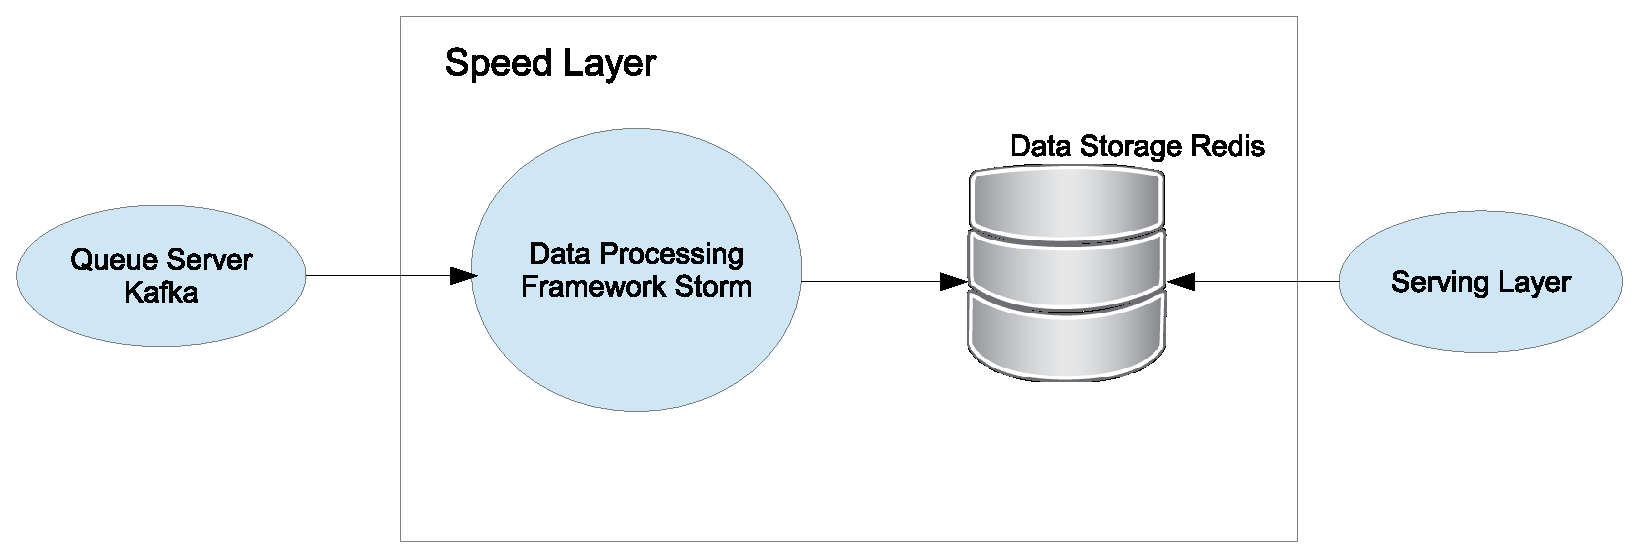
\includegraphics [width=1.0\textwidth]{images/SpeedLayerArchitecture}
  \caption{General structure of our system.}
  \label{fig:SpeedLayerArchitecture}
\end{figure}

\subsection{Data source}

The source of data, that is being processed, is the Kafka queue server \ref{subs:kafka}.
In its turn, it receives data from the outer sources, specifically from smartphones.
There are so far tens of thousends of smartphones, that use Menthal application and send data to the server.
Their number can grow arbitrarily, what requires in essence to have such a complex distributed server.
Smartphones send data to the server in small batches, that contain about fifty events, that happened since the last sending.
Kafka queue server stores this data temporarily, and tries to send it to all consumers, until they acknowledge delivery.
Our system is one of the consumers, and when it receives data, it starts processing. 

For each event type Kafka queue server maintains a dedicated topic.
It is possible then to subscribe for receiving of those events, that are needed for processing.
Events are sent as Avro objects \ref{subs:avro}, and contain meaningful information about what user does on the phone.
In our case we consider event types presented in the Table~\ref{table:event_types}.

\begin{table}[h]
\begin{tabular}{ | l | p{10cm} |}
    \hline
    AppInstall & Contains user id, app name and timestamp. Generated when the user installed a new application. \\ \hline
    AppSession & Contains user id, app name, timestamp and duration. Generated when the user has finished a session of using application. \\ \hline
    CallMissed & Contains user id, timestamp and contact hash. Generated when the user missed a call. Contact hash specifies a contact, that called. \\ \hline
    CallOutgoing & Contains user id, timestamp, contact hash and duration. Generated when the user finished an outgoing call. Contact hash specifies a contact, to that the call was addressed. \\ \hline
    CallReceived & Contains user id, timestamp, contact hash and duration. Generated when the user finished an incoming call. Contact hash specifies a contact, that called. \\ \hline
    DreamingStarted & Contains user id and timestamp. Generated when the phone gone to the dreaming mode. \\ \hline
    DreamingStopped & Contains user id and timestamp. Generated when the phone woke up from the dreaming mode. \\ \hline
    PhoneShutdown & Contains user id and timestamp. Generated when the phone goes off. \\ \hline
    ScreenOff & Contains user id and timestamp. Generated when the phone's screen goes off. \\ \hline
    ScreenOn & Contains user id and timestamp. Generated when the phone's screen goes on. \\ \hline
    ScreenUnlock & Contains user id and timestamp. Generated when the phone's screen is unlocked. \\ \hline
    SmsReceived & Contains user id,  timestamp, contact hash and message length. Generated when an sms is received. Contact hash specifies the contact, from that sms has come. \\ \hline
    SmsSent & Contains user id,  timestamp, contact hash and message length. Generated when an sms is sent. Contact hash specifies the contact, to that sms was sent. \\ \hline
    WindowStateChanged & Contains user id, timestamp, app name and window title. Generated when the new window becomes active. \\
    \hline
\end{tabular}
\caption{Event types and their descriptions}
\label{table:event_types}
\end{table}

\mnote{Kafka spout}
To obtain events from the Kafka queue server, we use \textit{Kafka spouts}.
Kafka spout is the class in the Storm's external class library, that allows to use Kafka queue server as a source of data for processing in the topology.
It listens for messages coming from Kafka in a particular topic.
Each such spout works in a distributed fashion, so that no matter how many events of a particular type will come, we can overcome this simply adding more machines to the cluster.

\subsection{Data processing}

The data processing framework Storm \ref{subs:storm} is the main component of the system.
It receives messages from Kafka queue server, and performs different computations on that data.
Its purpose is to provide different aggregatons on data coming from smartphones.
These aggregations are then stored in the storage system, and can be accessed by the Speed layer for answering queries.

The core of Storm framework is topology.
Topology describes the flow of computational logic.
It contains spouts and bolts, that represent data sources and data processing nodes, respectively.
We have already discussed Kafka spout, that we use for receiving data from the Kafka queue server.

Our topology has simple structure, but nevertheless has many nodes inside.
First of all, for each event type there is dedicated Kafka spout, that receives data from the Kafka queue server.
For that sake each Kafka spout is subscribed for a specific Kafka topic, corresponding to that event type.
When new message comes from the Kafka queue server, Storm runs particular spout on any available cluster node.

There is a dedicated bolt for each event type in our topology.
For each bolt we create a dedicated class, that performs particular processing, depending on what event type is it.
We use Storm's class \lstinline{BaseRichBolt} as a base class for all our bolts.
Our abstract class \lstinline{EventProcessingBolt}, that extends \lstinline{BaseRichBolt}, provides base functionality for all other bolts.
Every particular bolt class implements abstract method \lstinline{processEvent}, given in the class \lstinline{EventProcessingBolt}.
Such class hierarchy allows to add new event types for processing easily.
We just need to create new class, that inherits from \lstinline{EventProcessingBolt} and implements method \lstinline{processEvent}.

Class \lstinline{EventProcessingBolt} has a method \lstinline{getEventProcessingBoltByEventName}, that creates new bolt class by its name.
To achieve such functionality, class \lstinline{EventProcessingBolt} has protected field \lstinline{schemaName}.
It must be initialized in each derived class with the name of this particular event type.
This is useful again for the sake of extensibility, because it let's to leave code of topology initialization the same, no matter how many new event types we add for processing.
The main method of the \lstinline{EventProcessingBolt}, namely \lstinline{execute}, is presented on the Listing~\ref{listing:EventProcessingBolt_execute}.

\begin{lstlisting}[float=h, caption=The main method of the EventProcessingBolt., label=listing:EventProcessingBolt_execute, language=Java]
public void execute(Tuple tuple) {
  try {
    Schema schema = new Schema.Parser().parse(new File(schemaName + ".avsc"));
    DatumReader<GenericRecord> datumReader = new GenericDatumReader<GenericRecord>(schema);
    InputStream in = new ByteArrayInputStream((byte[])tuple.getValue(0));
    GenericRecord record = datumReader.read(null, DecoderFactory.get().jsonDecoder(schema, in));
    processEvent(record);
    _collector.emit(new Values(record));
  } catch (Exception e) {
    System.out.println("Exception raised!");
    System.out.println(e.getMessage());
  }
}
\end{lstlisting}

In the Line 3 we parse the schema of that particular event type.
Then in Lines 4-6 we parse input event to a \lstinline{GenericRecord} object using that schema.
\lstinline{GenericRecord} is an Avro class for representation of Avro objects in memory.
In the Line 7 we call abstract method \lstinline{processEvent}, that executes particular processing depending on what exact bolt class is it.

\lstinline{EventProcessingBolt} holds a reference to an interface \lstinline{EventAggregator}.
This interface provides method for processing all of event types that we consider.
Listing~\ref{listing:EventAggregator} shows the snippet from the definition of that interface.
We implemented exact class \lstinline{RedisEventAggregator} that realizes this interface.
As it states in its name, it works with Redis data storage.

\begin{lstlisting}[float=h, caption=The partial listing of the interface EventAggregator., label=listing:EventAggregator, language=Java]
public interface EventAggregator {
  void processAppSession(long userId, long time, long duration, String appName);
  void processCallMissed(long userId, long time, String contactHash, long timestamp);
  void processScreenOn(long userId, long time);
  void processSmsSent(long userId, long time, String contactHash, int msgLength);
  void processWindowStateChanged(long userId, long time, String appName, String windowTitle);
  ...
}
\end{lstlisting}

To make an example, let us consider one particular bolt class - \lstinline{AppSessionBolt}.
Listing~\ref{listing:AppSessionBolt} presents it.
In the constructor we initialize \lstinline{schemaName} with the name of this event type.
It is useful for creation of bolts by name.
In the method \lstinline{processEvent} we print out given record, then retrieve data fields from it, and pass them to a specific method of the \lstinline{eventAggregator} object, called \lstinline{processAppSession}.

\begin{lstlisting}[float=h, caption=Implementation of AppSessionBolt class., label=listing:AppSessionBolt, language=Java]
public class AppSessionBolt extends EventProcessingBolt {
  public AppSessionBolt() {
    schemaName = "app_session";
  }

  @Override
  protected void processEvent(GenericRecord record) {
    System.out.println(schemaName + "-Bolt: " + record.toString());
    long userId = (long)record.get("userId");
    long time = (long)record.get("time");
    long duration = (long)record.get("duration");
    String appName = record.get("appName").toString();
    eventAggregator.processAppSession(userId,time,duration,appName);
  }
}
\end{lstlisting}

On the events coming from smartphones we do different aggregations.
They will be then taken by the Serving layer for answering queries.
There are three types of aggregation, that we maintain in the data storage: counter, duration, and lenght.
Counter collects the number of events of any particular type.
Duration accumulates the total duration of the continuing action on the smartphone.
Length contains the total length of sms or whatsapp messages, etc.
There is a different logic of how to compute them for these three types of aggregations. 
For each aggregation we store four cases for different time intervals: last hour, last day, last week, last month.
Specifically, for each aggregations consists of two value: timestamp of the start of the current hour/day/week/month, and aggregation value itself.
Each time we update aggregation, that requires to recompute its starting timestamp.

\subsection{Data storage}

Data storage Redis \ref{subs:redis} keeps all results of computations.
These results are different aggregations, specifically counters, that are stored in the complex data model.
Redis provides simple access to save and then get that data.
Counters, saved in the Redis data storage can be then used by the Speed layer to merge them with the results of batch computations.

Redis is a key-value store, what defines the approach of storing data.
Each aggregations that we save to Redis is a list of two values: timestamp and value.

To work with aggregations in Redis we have developed a concrete class \lstinline{RedisEventAggregator}, that implements an interface \lstinline{EventAggregator}.
It works with the object of the type \lstinline{RedisProxy}, that we discribe later on in this section.
Each method of the class \lstinline{RedisEventAggregator} receives arguments as for example: user id, timestamp, app name, etc.
We then combine these values to a proper key name, that is present in Redis (or must be created on the first update).
Listing~\ref{listing:processAppSession} shows an example of key creation and passing it to \lstinline{RedisProxy}.

\begin{lstlisting}[float=h, caption=Example of key creation for aggregation update., label=listing:processAppSession, language=Java]
public void processAppSession(long userId, long time, long duration, String appName) {
  String key = String.format("app:%s:%s", appName, "sessions");
  redisProxy.incrementCounters(key, time);
  key = String.format("app:%s:%s", appName, "total_time");
  redisProxy.incrementDurations(key, time, duration);
  ...
\end{lstlisting}

We keep keys in Redis in the following way.
Each key is associated with the list, that has two elements.
The first one is the timestamp of the beginning of counting.
The second one is the value itself.
There are several examples of the keys in the Listing~\ref{listing:keysInRedis}.

\begin{lstlisting}[float=h, caption=Examples of the keys in Redis., label=listing:keysInRedis]
user:$user_id:$phone_hash:incoming_msg_count:count:hourly
user:$user_id:$phone_hash:incoming_msg_count:count:daily
user:$user_id:$phone_hash:incoming_msg_count:count:weekly
user:$user_id:$phone_hash:incoming_msg_count:count:monthly
user:$user_id:$phone_hash:outgoing_call_duration:duration:hourly
user:$user_id:$phone_hash:outgoing_call_duration:duration:daily
user:$user_id:$phone_hash:outgoing_call_duration:duration:weekly
user:$user_id:$phone_hash:outgoing_call_duration:duration:monthly
user:$user_id:$phone_hash:outgoing_msg_length:length:hourly
user:$user_id:$phone_hash:outgoing_msg_length:length:daily
user:$user_id:$phone_hash:outgoing_msg_length:length:weekly
user:$user_id:$phone_hash:outgoing_msg_length:length:monthly
\end{lstlisting}

To access Redis we use Jedis java library \cite{Jedis}.
It provides the the whole functionality, that Redis offers itself.
The class \lstinline{RedisProxy} contains all the communication with Redis.
It contains two fields, presentd on the Listing~\ref{listing:RedisProxyFields}.
They are the part of the Jedis library, and provide exact access to the Redis database.

\begin{lstlisting}[float=h, caption=Two main fields of the class RedisProxy., label=listing:RedisProxyFields, language=Java]
private final Jedis jedis;
private Pipeline pipeline;
\end{lstlisting}

\mnote{Pipeline}
We use \textit{pipelines} to communicate with Redis database.
Pipeline allows to combine several reqests to Redis into one batch, and send it altogether to the server through the network.
It reduces network congestion, and makes probability of race conditions on the server less.
\mnote{Transaction}
Inside of pipeline we use \textit{transaction} to tell Redis server, that we this set of commands must be executed as a one atomic command.
This is important to avoid race conditions, because many clients in the same time can try to access the same keys in the Redis database.
We demonstrate changing of the counter on the Listing~\ref{listing:incrementCounter}.

\begin{lstlisting}[float=h, caption=Example of updating counter aggregation in the Redis database., label=listing:incrementCounter, language=Java]
private void incrementCounter(DurationType durationType, CounterType counterType, String key, long time, long valueToIncrement) {
  key = String.format("%s:%s:%s", key, getCounterName(counterType), getDurationName(durationType));
  Boolean success = false;
  while (!success) {
    jedis.watch(key);
    List<String> value = jedis.lrange(key, 0, 1);
    pipeline = jedis.pipelined();
    pipeline.multi();
    Counter counter = new Counter(durationType, Long.parseLong(value.get(0)), Long.parseLong(value.get(1)));
    if (updateStartingTime(counter, time, 0))
      pipeline.lset(key, 0, Long.toString(counter.startTime));
    counter.value += valueToIncrement;
    pipeline.lset(key, 1, Long.toString(counter.value));
    success = (pipeline.exec() != null);
  }
  pipeline.sync();
}
\end{lstlisting}

We first generate in the Line 2 a proper key, that exactly exists in Redis, from a base key part.
Then we do do watching for values, that we want to retrieve and then change.
This is necessary to do, because this is the only way to protect the whole operation from race condition on the server side.
We get value of the counter in the Line 6.
Then in the Lines 7-8 we initialize pipeline and transaction.
In the Lines 9-12 we update retrieved counter in memory.
And in the Line 13 we set the new value of the counter into Redis server.
If in the time between watch and update of key's value it was accessed by other client, operation will fail, and we try to execute it again.

\section{Data flow}
General schema (picture)
3 pages

\section{Algorithms}

\section{Mapping to hardware}
how many servers, characteristics, data transferring
1 page

\authorsection{Aspects of implementation}{NO}
programming languages, etc.
